\documentclass[Lecture.tex]{subfiles}
\begin{document}
\section{6.1/6.2: Antiderivatives}

\begin{frame}{Antiderivatives}
  \begin{defn}
    Given a function, $f$, we say an {\it antiderivative} of $f$ is a function $F$ such that
    $$F^\prime(x) = f(x).$$
  \end{defn}
\end{frame}
\begin{frame}{Remarks}
  \begin{rmk}
    \begin{enumerate}
    \item<1->
      By the Fundamental Theorem of Calculus, given an antiderivative, $F$, of $f$,
      $$\int_a^b f(x)\dx{x} = \onslide<2->{\int_a^b F^\prime(x)\dx{x}} \onslide<3->{= F(b) - F(a).}$$
    \item<2->
      \onslide<4->{If $f$ admits an antiderivative, $F$, then for any $c \in \R$, $F(x) + c$ is also an antiderivative because}
      $$\onslide<4->{\ddx{x}\left(F(x) + c\right) =} \onslide<5->{\ddx{x}F(x) + \ddx{x}(c)} \onslide<6->{= f(x) + 0} \onslide<7->{= f(x).}$$
    \end{enumerate}
  \end{rmk}
\end{frame}

\subsection{Polynomials}

\begin{frame}{Monomials}
  For any monomial $f(x) = ax^n$, $0 \leq n$, an antiderivative of $f$ is
  $$F(x) = \onslide<2->{\frac{a}{n+1}x^{n+1} + c,\, c \in \R}$$
  \onslide<3->{since}
  $$\onslide<3->{F^\prime(x) =} \onslide<4->{\frac{a}{n+1}(n+1)x^n} \onslide<5->{= ax^n.}$$
\end{frame}

\begin{frame}{Polynomials}
  Since we know the antiderivative for a monomial, given a polynomial
  $$f(x) = \sum_{i=0}^n a_{n - i}x^{n-i}$$
  we have the antiderivative 
  $$F(x) = \sum_{i = 0}^n a_{n-i}\frac{1}{n - i + 1}x^{n - i + 1} + c,\, c \in \R.$$
\end{frame}
\begin{frame}{Polynomials (Cont.)}
  This follows from 
  \begin{eqnarray*}
    \onslide<2->{F^\prime(x) &=& \ddx{x}\left(\sum_{i = 0}^n a_{n-i}\frac{1}{n - i + 1}x^{n - i + 1} + c\right)\\}
    \onslide<3->{&=& \sum_{i = 0}^n \ddx{x}\left(a_{n-i}\frac{1}{n - i + 1}x^{n - i + 1}\right)\\}
    \onslide<4->{&=& \sum_{i = 0}^n a_{n-i}\frac{1}{n - i + 1}(n - i + 1)x^{n - i}\\}
    \onslide<5->{&=& \sum_{i = 0}^n a_{n - i}x^{n - i}\\}
    \onslide<6->{&=& f(x).}
  \end{eqnarray*}
\end{frame}

\begin{frame}{Example}
  Let $f(x) = 3x^2 + 2x + 5$.
  \onslide<2->{Then for any $c \in \R$, an antiderivative of $f$ is}
  $$\onslide<2->{F(x) =} \onslide<3->{3\frac{1}{3}x^3 + 2\frac{1}{2}x^2 + 5x + c} \onslide<4->{= x^3 + x^2 + 5x + c.}$$
  \onslide<5->{We can always check our solution:}
  $$\onslide<5->{F^\prime(x) =} \onslide<6->{\ddx{x}x^3 + \ddx{x}x^2 + 5\ddx{x}x} \onslide<7->{= 3x^2 + 2x + 5} \onslide<8->{= f(x).}$$
\end{frame}

\subsection{Exponentials}

\begin{frame}{Natural Exponentials}
  Let $P(x) = P_0e^{kx}$.
  Since $\ddx{x}e^{kx} = ke^{kx}$, we observe that 
  $$\onslide<2->{\ddx{x}\frac{P_0}{k}e^{kx} =} \onslide<3->{\frac{P_0}{k} \ddx{x}e^{kx}} \onslide<4->{= \frac{P_0}{k}\cdot k \cdot e^{kx}} \onslide<5->{= P_0 e^{kx}} \onslide<6->{= P(x).}$$
  \onslide<7->{
    This implies
    $$\frac{P_0}{k}e^{kx} + c,\, c \in \R$$
    is an antiderivative of $P(x)$.
  }
\end{frame}

\begin{frame}{Exponents with Arbitrary Base}
  If we want to integrate $P(x) = P_0a^x$, then we can rewrite as
  $$P(x) = P_0a^x = P_0e^{\ln(a)x}$$
  so that
  \begin{eqnarray*}
    \onslide<2->{\ddx{x} \frac{P_0}{\ln(a)}a^x &=&}
    \onslide<3->{\frac{P_0}{\ln(a)}\ddx{x}e^{\ln(a)x}\\}
    \onslide<4->{&=& \frac{P_0}{\ln(a)}\left(\ln(a)e^{\ln(a)x}\right)\\}
    \onslide<5->{&=& P_0a^x.}
  \end{eqnarray*}
  \onslide<6->{
    Therefore 
    $$\frac{P_0}{\ln(a)}a^x + c,\, c \in \R$$
    is an antiderivative of $P(x)$.
  }
\end{frame}
\subsection{The Indefinite Integral}

\begin{frame}{Definition}
  \begin{defn}
    If $f$ is a function with an antiderivative $F$, then the {\it indefinite integral} is the family of functions
    $$\int f(x)\dx{x} = F(x) + c$$
    where $c$ is a constant.
  \end{defn}

  \onslide<2->{
    \begin{rmk}
      Note that this immediately implies
      $$\ddx{x}\int f(x)\dx{x} = f(x).$$
    \end{rmk}
  }
\end{frame}

\begin{frame}{Properties of the Indefinite Integral}
  Assume that $\int f(x)\dx{x}$ and $\int g(x)\dx{x}$ exist.
  Then
  \begin{enumerate}
  \item<2->The indefinite integral of a sum is the sum of the indefinite integrals:
    $$\int f(x) \pm g(x)\dx{x} = \int f(x)\dx{x} \pm \int g(x)\dx{x}.$$
  \item<3->Constants pass through the indefnite integral:
    $$\int af(x)\dx{x} = a\int f(x)\dx{x},\, a \in \R.$$
  \end{enumerate}
\end{frame}

\subsection{Some Examples}
\begin{frame}{Examples}
  Integrate
  \begin{multicols}{4}
  \begin{enumerate}[(a)]
  \item<alert@2-3>
    $x^5$
  \item<alert@4-5>
    $t^8$
  \item<alert@6-9>
    $12x^3$
  \item<alert@10-14>
    $q^3 - 6q^2$
  \end{enumerate}
  \end{multicols}
  \vfill
  \begin{minipage}[t]{\linewidth}
    \only<2-3>{
      \begin{eqnarray*}
        \int x^5\dx{x} &=& \onslide<3->{\frac{1}{6}x^6 + c.}
      \end{eqnarray*}
    }
    \only<4-5>{
      \begin{eqnarray*}
        \int t^8\dx{t} &=& \onslide<5->{\frac{1}{9}x^9 + c.}
      \end{eqnarray*}
    }
    \only<6-9>{
      \begin{eqnarray*}
        \int 12x^3\dx{x} &=& 
        \onslide<7->{12\int x^3\dx{x}\\} 
        \onslide<8->{&=& 12\frac{1}{4}x^4 + c\\}
        \onslide<9->{&=& 3x^4 + c.}
      \end{eqnarray*}
    }
    \only<10-14>{
      \begin{eqnarray*}
        \int q^3 - 6q^2\dx{q} &=& 
      \onslide<11->{\int q^3\dx{q} - \int 6q^2\dx{q}\\}
      \onslide<12->{&=& \int q^3\dx{q} - 6\int q^2\dx{q}\\}
      \onslide<13->{&=& \frac{1}{4}q^4 - 6 \frac{1}{3}q^3 + c\\}
      \onslide<14->{&=& \frac{1}{4}q^4 - 2q^3 + c.\\}
      \end{eqnarray*}
      }
  \end{minipage}
\end{frame}

\begin{frame}{Example}
  Integrate
  $$12e^{0.2t}.$$
  
  \begin{eqnarray*}
    \onslide<2->{\int 12e^{0.2t}\dx{t} &=&}
    \onslide<3->{12 \int e^{\frac{t}{5}}\dx{t}}\\
    \onslide<4->{&=& 12\left(5e^{\frac{t}{5}}\right) + c\\}
    \onslide<5->{&=& 60e^{.02t} + c.}
  \end{eqnarray*}
\end{frame}

\subsection{Negative Exponents}
\begin{frame}{Negative Exponents}
  What is the indefinite integral of $\frac{1}{x^n}$?
  \onslide<2->{For $n < 1$, observe that}
  \begin{eqnarray*}
    \onslide<3->{\ddx{x}\left[\frac{1}{-n + 1}x^{-n + 1}\right] &=&}
    \onslide<4->{\frac{1}{-n + 1}\ddx{x}x^{-n + 1}}\\
    \onslide<5->{&=& \frac{1}{-n + 1}(-n + 1)x^{-n}}\\
    \onslide<6->{&=& x^{-n}\\}
    \onslide<7->{&=& \frac{1}{x^n}}
  \end{eqnarray*}
  \onslide<8->{
    Hence
    $$\int \frac{\dx{x}}{x^n} = \onslide<9->{\frac{1}{-n + 1}x^{-n + 1} + c} \onslide<10->{= \frac{1}{(-n + 1)x^{n - 1}} + c}$$
    }
\end{frame}

\begin{frame}{Example}
  Integrate 
  $$\frac{1}{x^3}.$$
  
  \begin{eqnarray*}
    \onslide<2->{\int \frac{\dx{x}}{x^3} =}
    \onslide<3->{\int x^{-3}\dx{x}\\}
    \onslide<4->{= \frac{1}{-2} x^{-2} + c\\}
    \onslide<5->{= \frac{-1}{2x^2} + c.}
  \end{eqnarray*}
\end{frame}

\begin{frame}{The Indefinite Integral of $\displaystyle{\frac{1}{x}}$}
  \begin{itemize}
    \item<1->
      When $n = 1$, the previous method fails because $1/(-n + 1)$ is undefined.
    \item<2->
      We observe that
      \onslide<3->{$$\ddx{x}\ln(x) = \frac{1}{x},$$}
      \onslide<4->{
        so we would expect
        $$\int \frac{\dx{x}}{x} = \ln(x) + c.$$
      }
    \item<5->
      This isn't quite true.
  \end{itemize}
  
\end{frame}

\begin{frame}{The Indefinite Integral of $\displaystyle{\frac{1}{x}}$ (Cont.)}
  Let $F(x)$ be an antiderivative of $1/x$.
  \onslide<2->{
    Since this function is continuous away from $x = 0$, we could ask: \\
    \begin{center}
      \parbox{0.8\linewidth}{
        What is the area between $1/x$ and the $x$-axis from $x = -2$ to $x = -1$?}
    \end{center}
  }
  \onslide<2->{
    \begin{center}
      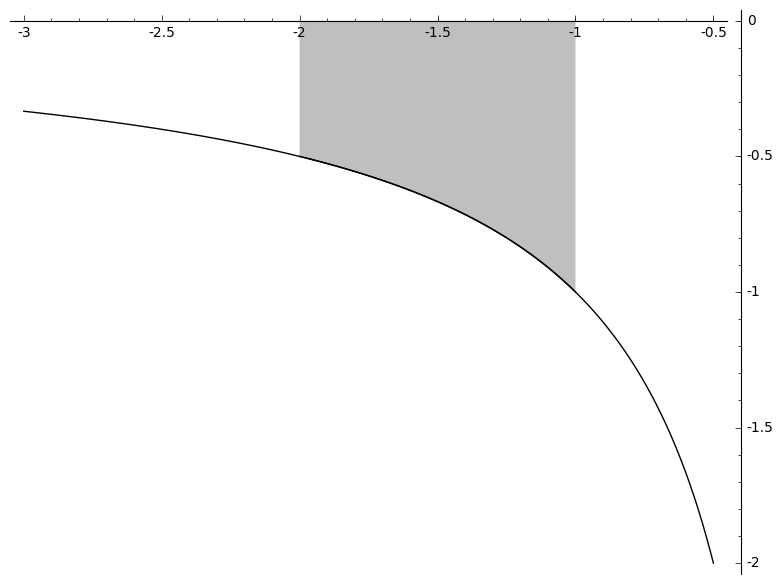
\includegraphics[scale=0.2]{areaUnderHyperbola}
    \end{center}
    }
  \onslide<3->{
    By the Fundamental Theorem of Calculus, this is
  }
  \onslide<4->{
    $$\int_{-2}^{-1} \frac{\dx{x}}{x} = F(-1) - F(-2).$$
  }
\end{frame}

\begin{frame}{The Indefinite Integral of $\displaystyle{\frac{1}{x}}$ (Cont.)}
  Since $\ln(x)$ is only defined for {\bf positive} values of $x$, $F(x) \neq \ln(x)$.
  We can fix this by taking $F(x) = \ln \abs{x}$.
  \onslide<2->{
    Recall that
    $$\abs{x} = \left\{
    \begin{array}{ll}
      x & \text{if}\ 0 \leq x,\\
      -x & \text{if}\ x < 0
    \end{array}
    \right. .$$
  }
  \onslide<3->{
    For $x < 0$ we have
    $$\ddx{x}\abs{x} = 
    \onslide<4->{\ddx{x}(-x)} 
    \onslide<5->{= -1.}$$
  }
  \onslide<6->{
    For $x > 0$ we have
    $$\ddx{x}\abs{x} = 
    \onslide<7->{\ddx{x}x}
    \onslide<8->{= 1.}$$
  }
\end{frame}

\begin{frame}{The Indefinite Integral of $\displaystyle{\frac{1}{x}}$ (Cont.)}
  By the Chain Rule,
  \begin{eqnarray*}
    \onslide<2->{\ddx{x} \ln \abs{x} &=&}
    \onslide<3->{\frac{\ddx{x}\abs{x}}{\abs{x}}\\}
    \onslide<4->{&=& \left\{
  \begin{array}{ll}
    \frac{1}{x} & \text{if}\ 0 < x\\
    \frac{-1}{-x} = \frac{1}{x} & \text{if}\ x < 0.
  \end{array}
  \right.\\}
    \onslide<5->{&=& \frac{1}{x}.}
  \end{eqnarray*}
  \onslide<6->{
    Therefore
    $$\int \frac{\dx{x}}{x} = \ln\abs{x} + c.$$
  }
\end{frame}
\end{document}
